\documentclass[letterpaper]{book}
\usepackage{makeidx}
\usepackage{fancyhdr}
\usepackage{graphicx}
\usepackage{multicol}
\usepackage{float}
\usepackage{textcomp}
\usepackage{alltt}
\usepackage{times}
\usepackage{ifpdf}
\ifpdf
\usepackage[pdftex,
            pagebackref=true,
            colorlinks=true,
            linkcolor=blue,
            unicode
           ]{hyperref}
\else
\usepackage[ps2pdf,
            pagebackref=true,
            colorlinks=true,
            linkcolor=blue,
            unicode
           ]{hyperref}
\usepackage{pspicture}
\fi
\usepackage[utf8]{inputenc}
\usepackage{doxygen}
\makeindex
\setcounter{tocdepth}{3}
\renewcommand{\footrulewidth}{0.4pt}
\begin{document}
\begin{titlepage}
\vspace*{7cm}
\begin{center}
{\Large Polynomial Manipulation }\\
\vspace*{1cm}
{\large Generated by Doxygen 1.5.6}\\
\vspace*{0.5cm}
{\small Tue Oct 18 10:48:11 2011}\\
\end{center}
\end{titlepage}
\clearemptydoublepage
\pagenumbering{roman}
\tableofcontents
\clearemptydoublepage
\pagenumbering{arabic}
\chapter{Main Page}
\label{index}\hypertarget{index}{}\hyperlink{classPolynomial}{Polynomial} Manipulation Program. MCS 360 Fall 2011 Project 2\hypertarget{index_Overview}{}\section{Overview}\label{index_Overview}
This is a menu driven program which allows a user to input polynomials of arbitrary length and degree. Operations including multiplication and addition of polynomials is available for any previously defined polynomials, and all results are saved for future use.\hypertarget{index_Use}{}\section{Use}\label{index_Use}
To begin, add polynomials to work with. The input routine first asks for the number of terms in the polynomial, and then for each term requests a degree and a coefficient. The resulting polynomial is the sum of the given terms. Polynomials are always stored and displayed in ascending degree, and reduced by combining like terms.

Once polynomials have been added to the system, they may be recalled by numbers (in order of creation). Unneeded terms may be deleted when the number of polynomials in memory makes using the system unpleasant.

Polynomials may be added, subtracted, or multiplied. A special case for multiplying by a scalar is allowed, which is simply a constant polynomial under the hood.\hypertarget{index_Cavaets}{}\section{Cavaets}\label{index_Cavaets}
It should be noted that multiplying two very large polynomials (number of terms) is a time consuming process O(n$^\wedge$2), while addition and evaluation at a point are O(n).

Scalar multiplication cowardly refuses to multiply by zero. The user is welcome to solve this himself.

Coefficients are represented using machine doubles. Repeated multiplication or addition will result in {\em inf\/} as a value. Precision is inversely proportional to magnitude for doubles. No attempt to minimize errors was made.\hypertarget{index_History}{}\section{History}\label{index_History}
This was the second programming project for MCS 360 at UIC in Fall 2011. Substantial portions of the menu system and the user input routines were adapted from the first project. Any future revisions would do well to modularize further the menu object, and possibly allow reassignment of the istream/ostream for the \hyperlink{classInputValidator}{InputValidator}. 
\chapter{Class Index}
\section{Class List}
Here are the classes, structs, unions and interfaces with brief descriptions:\begin{CompactList}
\item\contentsline{section}{\hyperlink{classInputValidator}{InputValidator$<$ T $>$} }{\pageref{classInputValidator}}{}
\item\contentsline{section}{\hyperlink{classPolynomial}{Polynomial} (\hyperlink{classPolynomial}{Polynomial} as a linked list of terms )}{\pageref{classPolynomial}}{}
\item\contentsline{section}{\hyperlink{classPolynomialMenu}{PolynomialMenu} (The main program logic, contains a vector of Polynomials, means to generate them, means to add and multiply existing polynomials, handles user input/output, and displays the menu and the polynomials in the vector )}{\pageref{classPolynomialMenu}}{}
\end{CompactList}

\chapter{File Index}
\section{File List}
Here is a list of all documented files with brief descriptions:\begin{CompactList}
\item\contentsline{section}{\hyperlink{InputValidator_8h}{InputValidator.h} (A templated type validator from cin/cout )}{\pageref{InputValidator_8h}}{}
\item\contentsline{section}{\hyperlink{main_8cc}{main.cc} (Start menu system )}{\pageref{main_8cc}}{}
\item\contentsline{section}{\hyperlink{menu_8cc}{menu.cc} (Implement the menu logic )}{\pageref{menu_8cc}}{}
\item\contentsline{section}{\hyperlink{menu_8h}{menu.h} (Definition of the polynomial menu system )}{\pageref{menu_8h}}{}
\item\contentsline{section}{\hyperlink{poly_8cc}{poly.cc} (Implementation for the polynomial class )}{\pageref{poly_8cc}}{}
\item\contentsline{section}{\hyperlink{poly_8h}{poly.h} (Declaration of the polynomial class )}{\pageref{poly_8h}}{}
\end{CompactList}

\chapter{Class Documentation}
\hypertarget{classInputValidator}{
\section{InputValidator$<$ T $>$ Class Template Reference}
\label{classInputValidator}\index{InputValidator@{InputValidator}}
}
{\tt \#include $<$InputValidator.h$>$}

Collaboration diagram for InputValidator$<$ T $>$:\nopagebreak
\begin{figure}[H]
\begin{center}
\leavevmode
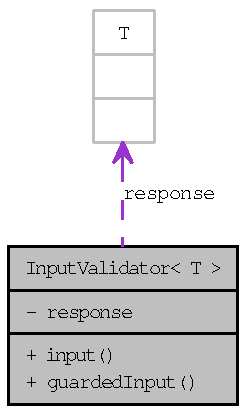
\includegraphics[width=77pt]{classInputValidator__coll__graph}
\end{center}
\end{figure}
\subsection*{Public Member Functions}
\begin{CompactItemize}
\item 
T \hyperlink{classInputValidator_4d554feb8dc41f8990e62a34d2678574}{input} (std::string prompt)
\begin{CompactList}\small\item\em checks that response was received from cin. \item\end{CompactList}\item 
T \hyperlink{classInputValidator_c00d4a6ca94d48eb3c8b9e2b57b31950}{guardedInput} (std::string prompt, std::string reprompt, T guard)
\end{CompactItemize}


\subsection{Detailed Description}
\subsubsection*{template$<$typename T$>$ class InputValidator$<$ T $>$}

\begin{Desc}
\item[Template Parameters:]
\begin{description}
\item[{\em T}]is the type of input to look for\end{description}
\end{Desc}
T must provide the equality operator This is error prone with doubles so some external checks are in order 

Definition at line 25 of file InputValidator.h.

\subsection{Member Function Documentation}
\hypertarget{classInputValidator_4d554feb8dc41f8990e62a34d2678574}{
\index{InputValidator@{InputValidator}!input@{input}}
\index{input@{input}!InputValidator@{InputValidator}}
\subsubsection[input]{\setlength{\rightskip}{0pt plus 5cm}template$<$typename T$>$ T {\bf InputValidator}$<$ T $>$::input (std::string {\em prompt})\hspace{0.3cm}{\tt  \mbox{[}inline\mbox{]}}}}
\label{classInputValidator_4d554feb8dc41f8990e62a34d2678574}


checks that response was received from cin. 

\hyperlink{classInputValidator_4d554feb8dc41f8990e62a34d2678574}{input()} presents a prompt and returns response. \begin{Desc}
\item[Parameters:]
\begin{description}
\item[{\em prompt}]is a string to present before reading \end{description}
\end{Desc}
\begin{Desc}
\item[Returns:]response \end{Desc}


Definition at line 33 of file InputValidator.h.

\begin{Code}\begin{verbatim}33                             {
34     std::cin.clear();
35     std::cout<<prompt;
36     std::cin>>response;
37     if(std::cin.fail())
38       return input(prompt);
39     else
40       return response;
41   }
\end{verbatim}
\end{Code}




Here is the caller graph for this function:\nopagebreak
\begin{figure}[H]
\begin{center}
\leavevmode
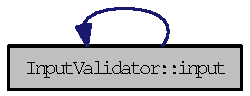
\includegraphics[width=78pt]{classInputValidator_4d554feb8dc41f8990e62a34d2678574_icgraph}
\end{center}
\end{figure}
\hypertarget{classInputValidator_c00d4a6ca94d48eb3c8b9e2b57b31950}{
\index{InputValidator@{InputValidator}!guardedInput@{guardedInput}}
\index{guardedInput@{guardedInput}!InputValidator@{InputValidator}}
\subsubsection[guardedInput]{\setlength{\rightskip}{0pt plus 5cm}template$<$typename T$>$ T {\bf InputValidator}$<$ T $>$::guardedInput (std::string {\em prompt}, \/  std::string {\em reprompt}, \/  T {\em guard})\hspace{0.3cm}{\tt  \mbox{[}inline\mbox{]}}}}
\label{classInputValidator_c00d4a6ca94d48eb3c8b9e2b57b31950}


guardedInput presents a prompt and ensures some new information was given. Allows a custom reprompt.

\begin{Desc}
\item[Parameters:]
\begin{description}
\item[{\em prompt}]is the string to present prior to input \item[{\em reprompt}]is a corrective hint \item[{\em guard}]is a known bad value that should not be set \end{description}
\end{Desc}
\begin{Desc}
\item[Postcondition:]response is not guard. \end{Desc}
\begin{Desc}
\item[Returns:]response \end{Desc}


Definition at line 52 of file InputValidator.h.

\begin{Code}\begin{verbatim}52                                                                {
53     response = guard;
54     while(response==guard){
55       std::cout<<prompt;
56       std::cin>>response;
57       if(std::cin.fail()){
58     std::cout<<reprompt;
59     response=guard;
60     std::cin.clear();
61     std::cin.ignore(100,'\n');
62       }
63     }
64     return response;
65   }
\end{verbatim}
\end{Code}




The documentation for this class was generated from the following file:\begin{CompactItemize}
\item 
\hyperlink{InputValidator_8h}{InputValidator.h}\end{CompactItemize}

\hypertarget{classPolynomial}{
\section{Polynomial Class Reference}
\label{classPolynomial}\index{Polynomial@{Polynomial}}
}
represents the polynomial as a linked list of terms  


{\tt \#include $<$poly.h$>$}

Collaboration diagram for Polynomial:\nopagebreak
\begin{figure}[H]
\begin{center}
\leavevmode
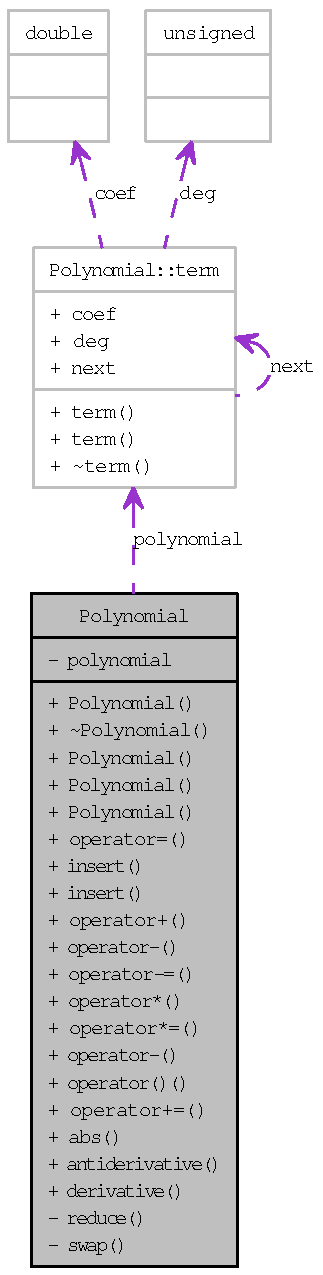
\includegraphics[height=400pt]{classPolynomial__coll__graph}
\end{center}
\end{figure}
\subsection*{Public Member Functions}
\begin{CompactItemize}
\item 
\hyperlink{classPolynomial_961dec5c0727f03e5273f74a345dfbb6}{Polynomial} ()
\item 
\hyperlink{classPolynomial_96130e913259691bd82b7d910d586169}{$\sim$Polynomial} ()
\item 
\hyperlink{classPolynomial_fa571a95bc93973b6727e4bdbda7a43d}{Polynomial} (const \hyperlink{classPolynomial}{Polynomial} \&rhs)
\item 
\hyperlink{classPolynomial_91d11d1fc330f36c78de3527692e5bf2}{Polynomial} (const double rhs)
\item 
\hyperlink{classPolynomial_2fdf4061d1783d216de7a6c24768cef0}{Polynomial} (const double coef, const unsigned deg)
\item 
\hyperlink{classPolynomial}{Polynomial} \& \hyperlink{classPolynomial_76d719fc2a24feb250ee2dbddcb6c8bb}{operator=} (const \hyperlink{classPolynomial}{Polynomial} \&rhs)
\item 
void \hyperlink{classPolynomial_b141080a5700f160d4bd1d68cecfd50f}{insert} (term $\ast$t)
\item 
void \hyperlink{classPolynomial_47a8de184c159d413235dbb3a192554d}{insert} (double coef, unsigned deg)
\item 
const \hyperlink{classPolynomial}{Polynomial} \hyperlink{classPolynomial_74b75f9d3274a46baa91c84fc5aad1f8}{operator+} (const \hyperlink{classPolynomial}{Polynomial} \&rhs) const 
\item 
\hyperlink{classPolynomial}{Polynomial} \hyperlink{classPolynomial_cff0b8a8c385f43f9d57c80ee925d858}{operator-} (const \hyperlink{classPolynomial}{Polynomial} \&rhs) const 
\item 
\hyperlink{classPolynomial}{Polynomial} \& \hyperlink{classPolynomial_f89937a0177661ce28acabddc5a9cfaf}{operator-=} (const \hyperlink{classPolynomial}{Polynomial} \&rhs)
\item 
\hyperlink{classPolynomial}{Polynomial} \hyperlink{classPolynomial_1e00f25b4de1d335f437749c7bd93ac9}{operator$\ast$} (const \hyperlink{classPolynomial}{Polynomial} \&rhs) const 
\item 
\hyperlink{classPolynomial}{Polynomial} \& \hyperlink{classPolynomial_cd98d02bf606b1f1cd7503d7e3b295a6}{operator$\ast$=} (const \hyperlink{classPolynomial}{Polynomial} \&rhs)
\item 
\hyperlink{classPolynomial}{Polynomial} \hyperlink{classPolynomial_d052b311f23798bf5136bd7444fd91d2}{operator-} () const 
\item 
double \hyperlink{classPolynomial_c6eae37f11f87b541fa430de3643a31a}{operator()} (double a) const 
\item 
\hyperlink{classPolynomial}{Polynomial} \& \hyperlink{classPolynomial_2ceb25a673d4c03b346595639ade0981}{operator+=} (const \hyperlink{classPolynomial}{Polynomial} \&rhs)
\item 
\hyperlink{classPolynomial}{Polynomial} \hyperlink{classPolynomial_1e8588431fc5799e62bba71368a7234d}{abs} () const 
\item 
\hyperlink{classPolynomial}{Polynomial} \hyperlink{classPolynomial_4db9e4f680c52fb8af45f3ae985a4055}{antiderivative} () const 
\item 
\hyperlink{classPolynomial}{Polynomial} \hyperlink{classPolynomial_aef1ed2dbc29d419c58c6d61b35853c3}{derivative} () const 
\end{CompactItemize}
\subsection*{Friends}
\begin{CompactItemize}
\item 
std::istream \& \hyperlink{classPolynomial_1446b464245742ccedeacb27fd794bab}{operator$>$$>$} (std::istream \&is, \hyperlink{classPolynomial}{Polynomial} \&p)
\item 
std::ostream \& \hyperlink{classPolynomial_f1fdf53b29100b084772816cb9ecc8ac}{operator$<$$<$} (std::ostream \&os, const \hyperlink{classPolynomial}{Polynomial} \&p)
\end{CompactItemize}
\subsection*{Classes}
\begin{CompactItemize}
\item 
class \textbf{term}
\end{CompactItemize}


\subsection{Detailed Description}
represents the polynomial as a linked list of terms 

Definition at line 14 of file poly.h.

\subsection{Constructor \& Destructor Documentation}
\hypertarget{classPolynomial_961dec5c0727f03e5273f74a345dfbb6}{
\index{Polynomial@{Polynomial}!Polynomial@{Polynomial}}
\index{Polynomial@{Polynomial}!Polynomial@{Polynomial}}
\subsubsection[Polynomial]{\setlength{\rightskip}{0pt plus 5cm}Polynomial::Polynomial ()}}
\label{classPolynomial_961dec5c0727f03e5273f74a345dfbb6}


default constructor, gives the zero polynomial

default constructor, returns a zero polynomial 

Definition at line 33 of file poly.cc.

\begin{Code}\begin{verbatim}33                       {
34   // get the zero term
35   polynomial = new term(0.0, 0);
36 }
\end{verbatim}
\end{Code}


\hypertarget{classPolynomial_96130e913259691bd82b7d910d586169}{
\index{Polynomial@{Polynomial}!$\sim$Polynomial@{$\sim$Polynomial}}
\index{$\sim$Polynomial@{$\sim$Polynomial}!Polynomial@{Polynomial}}
\subsubsection[$\sim$Polynomial]{\setlength{\rightskip}{0pt plus 5cm}Polynomial::$\sim$Polynomial ()}}
\label{classPolynomial_96130e913259691bd82b7d910d586169}


default destructor

delete each term before expiring 

Definition at line 47 of file poly.cc.

\begin{Code}\begin{verbatim}47                        {
48   term * t;
49   while(polynomial){
50     t = polynomial;
51     polynomial = t->next;
52     delete t;
53   }
54 }
\end{verbatim}
\end{Code}


\hypertarget{classPolynomial_fa571a95bc93973b6727e4bdbda7a43d}{
\index{Polynomial@{Polynomial}!Polynomial@{Polynomial}}
\index{Polynomial@{Polynomial}!Polynomial@{Polynomial}}
\subsubsection[Polynomial]{\setlength{\rightskip}{0pt plus 5cm}Polynomial::Polynomial (const {\bf Polynomial} \& {\em rhs})}}
\label{classPolynomial_fa571a95bc93973b6727e4bdbda7a43d}


copy constructor 

Definition at line 268 of file poly.cc.

References insert(), and polynomial.

\begin{Code}\begin{verbatim}268                                            {
269   term * t;
270   // initialize
271   polynomial = new term();
272   // copy
273   t = rhs.polynomial;
274   while(t){
275     insert(t->coef, t->deg);
276     t = t->next;
277   }
278 }
\end{verbatim}
\end{Code}




Here is the call graph for this function:\nopagebreak
\begin{figure}[H]
\begin{center}
\leavevmode
\includegraphics[width=154pt]{classPolynomial_fa571a95bc93973b6727e4bdbda7a43d_cgraph}
\end{center}
\end{figure}
\hypertarget{classPolynomial_91d11d1fc330f36c78de3527692e5bf2}{
\index{Polynomial@{Polynomial}!Polynomial@{Polynomial}}
\index{Polynomial@{Polynomial}!Polynomial@{Polynomial}}
\subsubsection[Polynomial]{\setlength{\rightskip}{0pt plus 5cm}Polynomial::Polynomial (const double {\em rhs})}}
\label{classPolynomial_91d11d1fc330f36c78de3527692e5bf2}


allow promotions 

Definition at line 38 of file poly.cc.

\begin{Code}\begin{verbatim}38                                       {
39   polynomial = new term(rhs,0);
40 }
\end{verbatim}
\end{Code}


\hypertarget{classPolynomial_2fdf4061d1783d216de7a6c24768cef0}{
\index{Polynomial@{Polynomial}!Polynomial@{Polynomial}}
\index{Polynomial@{Polynomial}!Polynomial@{Polynomial}}
\subsubsection[Polynomial]{\setlength{\rightskip}{0pt plus 5cm}Polynomial::Polynomial (const double {\em coef}, \/  const unsigned {\em deg})}}
\label{classPolynomial_2fdf4061d1783d216de7a6c24768cef0}


allow construction of monomials 

Definition at line 42 of file poly.cc.

\begin{Code}\begin{verbatim}42                                                            {
43   polynomial = new term(coef, deg);
44 }
\end{verbatim}
\end{Code}




\subsection{Member Function Documentation}
\hypertarget{classPolynomial_76d719fc2a24feb250ee2dbddcb6c8bb}{
\index{Polynomial@{Polynomial}!operator=@{operator=}}
\index{operator=@{operator=}!Polynomial@{Polynomial}}
\subsubsection[operator=]{\setlength{\rightskip}{0pt plus 5cm}{\bf Polynomial} \& Polynomial::operator= (const {\bf Polynomial} \& {\em rhs})}}
\label{classPolynomial_76d719fc2a24feb250ee2dbddcb6c8bb}


assignment operator 

Definition at line 259 of file poly.cc.

\begin{Code}\begin{verbatim}259                                                        {
260   if(this != &rhs){
261     Polynomial tmp(rhs);
262     swap(tmp);
263   }
264  return *this;
265 }
\end{verbatim}
\end{Code}


\hypertarget{classPolynomial_b141080a5700f160d4bd1d68cecfd50f}{
\index{Polynomial@{Polynomial}!insert@{insert}}
\index{insert@{insert}!Polynomial@{Polynomial}}
\subsubsection[insert]{\setlength{\rightskip}{0pt plus 5cm}void Polynomial::insert (term $\ast$ {\em t})}}
\label{classPolynomial_b141080a5700f160d4bd1d68cecfd50f}


add a term to the list

insert : add to list \& reduce insert is in degree order polynomial is maintained in sorted order reduce only combines like terms. 

Definition at line 61 of file poly.cc.

\begin{Code}\begin{verbatim}61                                {
62   term * u = polynomial;
63   term * prev = NULL;
64   while(u->next && ( t->deg > u->deg)){
65     prev = u;
66     u = u->next;
67   }
68   if (u == polynomial && !(t->deg >= u->deg)){
69     //still at head of list, and t is not bigger
70     polynomial = t;
71     t->next = u;
72   }  else if (t->deg > u->deg){
73     // got to end of list
74     u->next = t;
75   }
76   else {
77     // in the middle
78     t->next = u;;
79     if(prev)
80       prev->next = t;
81     else polynomial = t;
82   }
83   reduce();
84   return;
85 }
\end{verbatim}
\end{Code}




Here is the caller graph for this function:\nopagebreak
\begin{figure}[H]
\begin{center}
\leavevmode
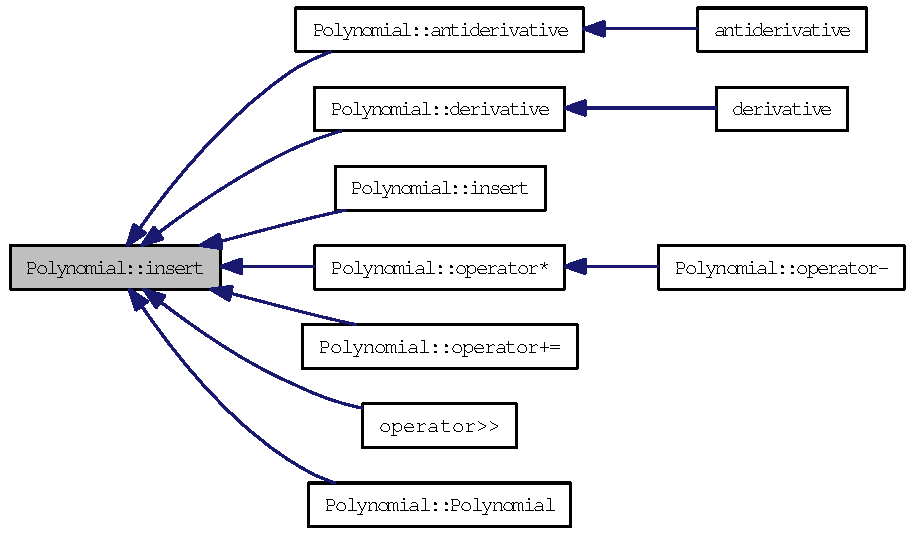
\includegraphics[width=237pt]{classPolynomial_b141080a5700f160d4bd1d68cecfd50f_icgraph}
\end{center}
\end{figure}
\hypertarget{classPolynomial_47a8de184c159d413235dbb3a192554d}{
\index{Polynomial@{Polynomial}!insert@{insert}}
\index{insert@{insert}!Polynomial@{Polynomial}}
\subsubsection[insert]{\setlength{\rightskip}{0pt plus 5cm}void Polynomial::insert (double {\em coef} = {\tt 0}, \/  unsigned {\em deg} = {\tt 0})}}
\label{classPolynomial_47a8de184c159d413235dbb3a192554d}


insert : doesn't require user to call constructor for term 

Definition at line 88 of file poly.cc.

References insert().

\begin{Code}\begin{verbatim}88                                                     {
89   term * t = new term(coef, deg);
90   insert(t);
91   return;
92 }
\end{verbatim}
\end{Code}




Here is the call graph for this function:\nopagebreak
\begin{figure}[H]
\begin{center}
\leavevmode
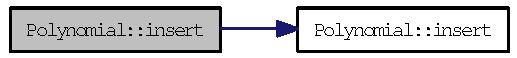
\includegraphics[width=142pt]{classPolynomial_47a8de184c159d413235dbb3a192554d_cgraph}
\end{center}
\end{figure}
\hypertarget{classPolynomial_74b75f9d3274a46baa91c84fc5aad1f8}{
\index{Polynomial@{Polynomial}!operator+@{operator+}}
\index{operator+@{operator+}!Polynomial@{Polynomial}}
\subsubsection[operator+]{\setlength{\rightskip}{0pt plus 5cm}const {\bf Polynomial} Polynomial::operator+ (const {\bf Polynomial} \& {\em rhs}) const}}
\label{classPolynomial_74b75f9d3274a46baa91c84fc5aad1f8}


addition operator 

Definition at line 108 of file poly.cc.

\begin{Code}\begin{verbatim}109 {
110   Polynomial tmp(*this);
111   tmp += rhs;
112   return tmp;
113 }
\end{verbatim}
\end{Code}


\hypertarget{classPolynomial_cff0b8a8c385f43f9d57c80ee925d858}{
\index{Polynomial@{Polynomial}!operator-@{operator-}}
\index{operator-@{operator-}!Polynomial@{Polynomial}}
\subsubsection[operator-]{\setlength{\rightskip}{0pt plus 5cm}{\bf Polynomial} Polynomial::operator- (const {\bf Polynomial} \& {\em rhs}) const}}
\label{classPolynomial_cff0b8a8c385f43f9d57c80ee925d858}


subtraction operator

subtraction operator add -rhs 

Definition at line 187 of file poly.cc.

\begin{Code}\begin{verbatim}187                                                             {
188   return *this + -rhs;
189 }
\end{verbatim}
\end{Code}


\hypertarget{classPolynomial_f89937a0177661ce28acabddc5a9cfaf}{
\index{Polynomial@{Polynomial}!operator-=@{operator-=}}
\index{operator-=@{operator-=}!Polynomial@{Polynomial}}
\subsubsection[operator-=]{\setlength{\rightskip}{0pt plus 5cm}{\bf Polynomial} \& Polynomial::operator-= (const {\bf Polynomial} \& {\em rhs})}}
\label{classPolynomial_f89937a0177661ce28acabddc5a9cfaf}


subtraction/assignment operator 

Definition at line 191 of file poly.cc.

\begin{Code}\begin{verbatim}191                                                         {
192   *this += (-rhs);
193   return *this;
194 }
\end{verbatim}
\end{Code}


\hypertarget{classPolynomial_1e00f25b4de1d335f437749c7bd93ac9}{
\index{Polynomial@{Polynomial}!operator$\ast$@{operator$\ast$}}
\index{operator$\ast$@{operator$\ast$}!Polynomial@{Polynomial}}
\subsubsection[operator$\ast$]{\setlength{\rightskip}{0pt plus 5cm}{\bf Polynomial} Polynomial::operator$\ast$ (const {\bf Polynomial} \& {\em rhs}) const}}
\label{classPolynomial_1e00f25b4de1d335f437749c7bd93ac9}


multiplication operator 

Definition at line 154 of file poly.cc.

References insert().

\begin{Code}\begin{verbatim}154                                {
155   // for each term in rhs
156   // multiply terms by coef and raise power by deg
157   Polynomial p;
158   term * u;
159   term * t = rhs.polynomial;
160   while (t) {
161     u = polynomial;
162     while(u){
163       p.insert(u->coef * t->coef, u->deg + t->deg);
164       u = u->next;
165     }
166     t = t->next;
167   }
168   return p;
169 }
\end{verbatim}
\end{Code}




Here is the call graph for this function:\nopagebreak
\begin{figure}[H]
\begin{center}
\leavevmode
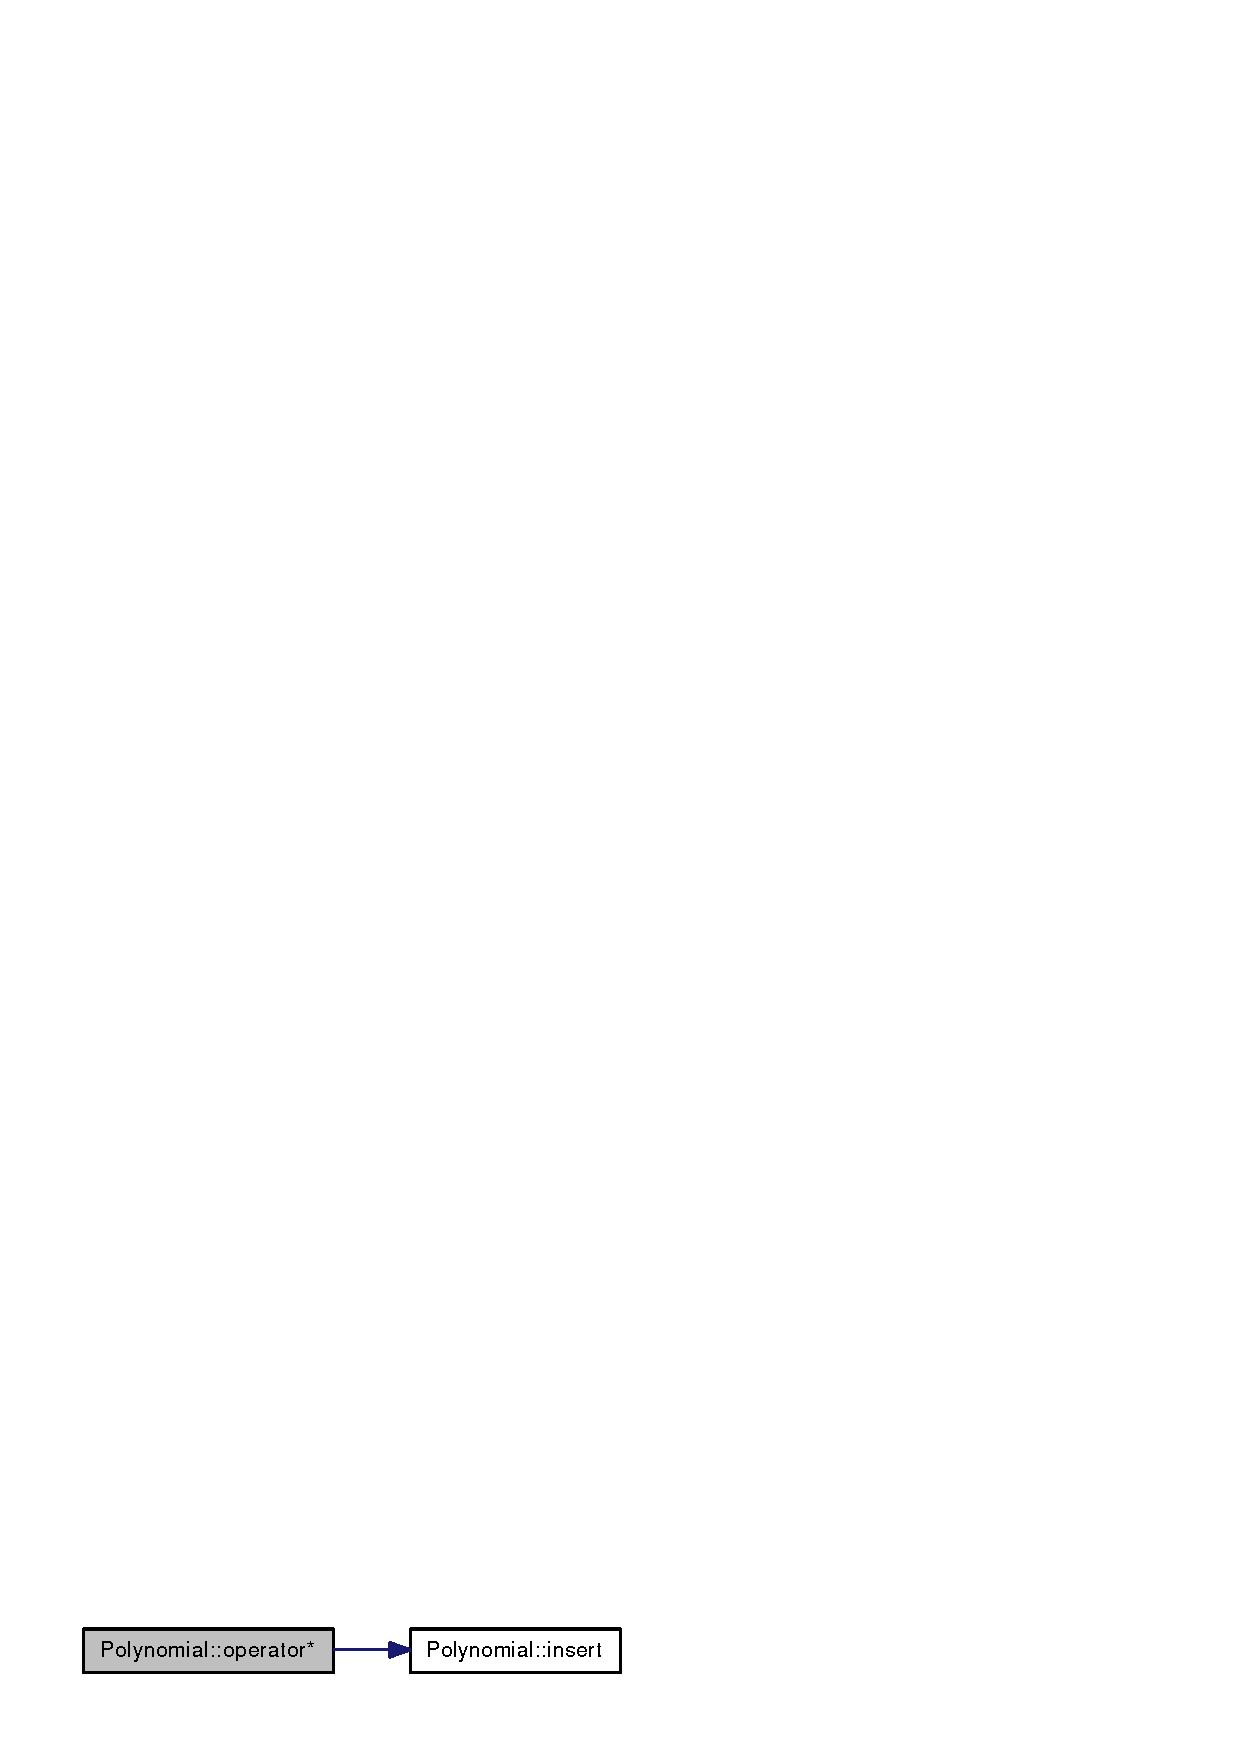
\includegraphics[width=151pt]{classPolynomial_1e00f25b4de1d335f437749c7bd93ac9_cgraph}
\end{center}
\end{figure}


Here is the caller graph for this function:\nopagebreak
\begin{figure}[H]
\begin{center}
\leavevmode
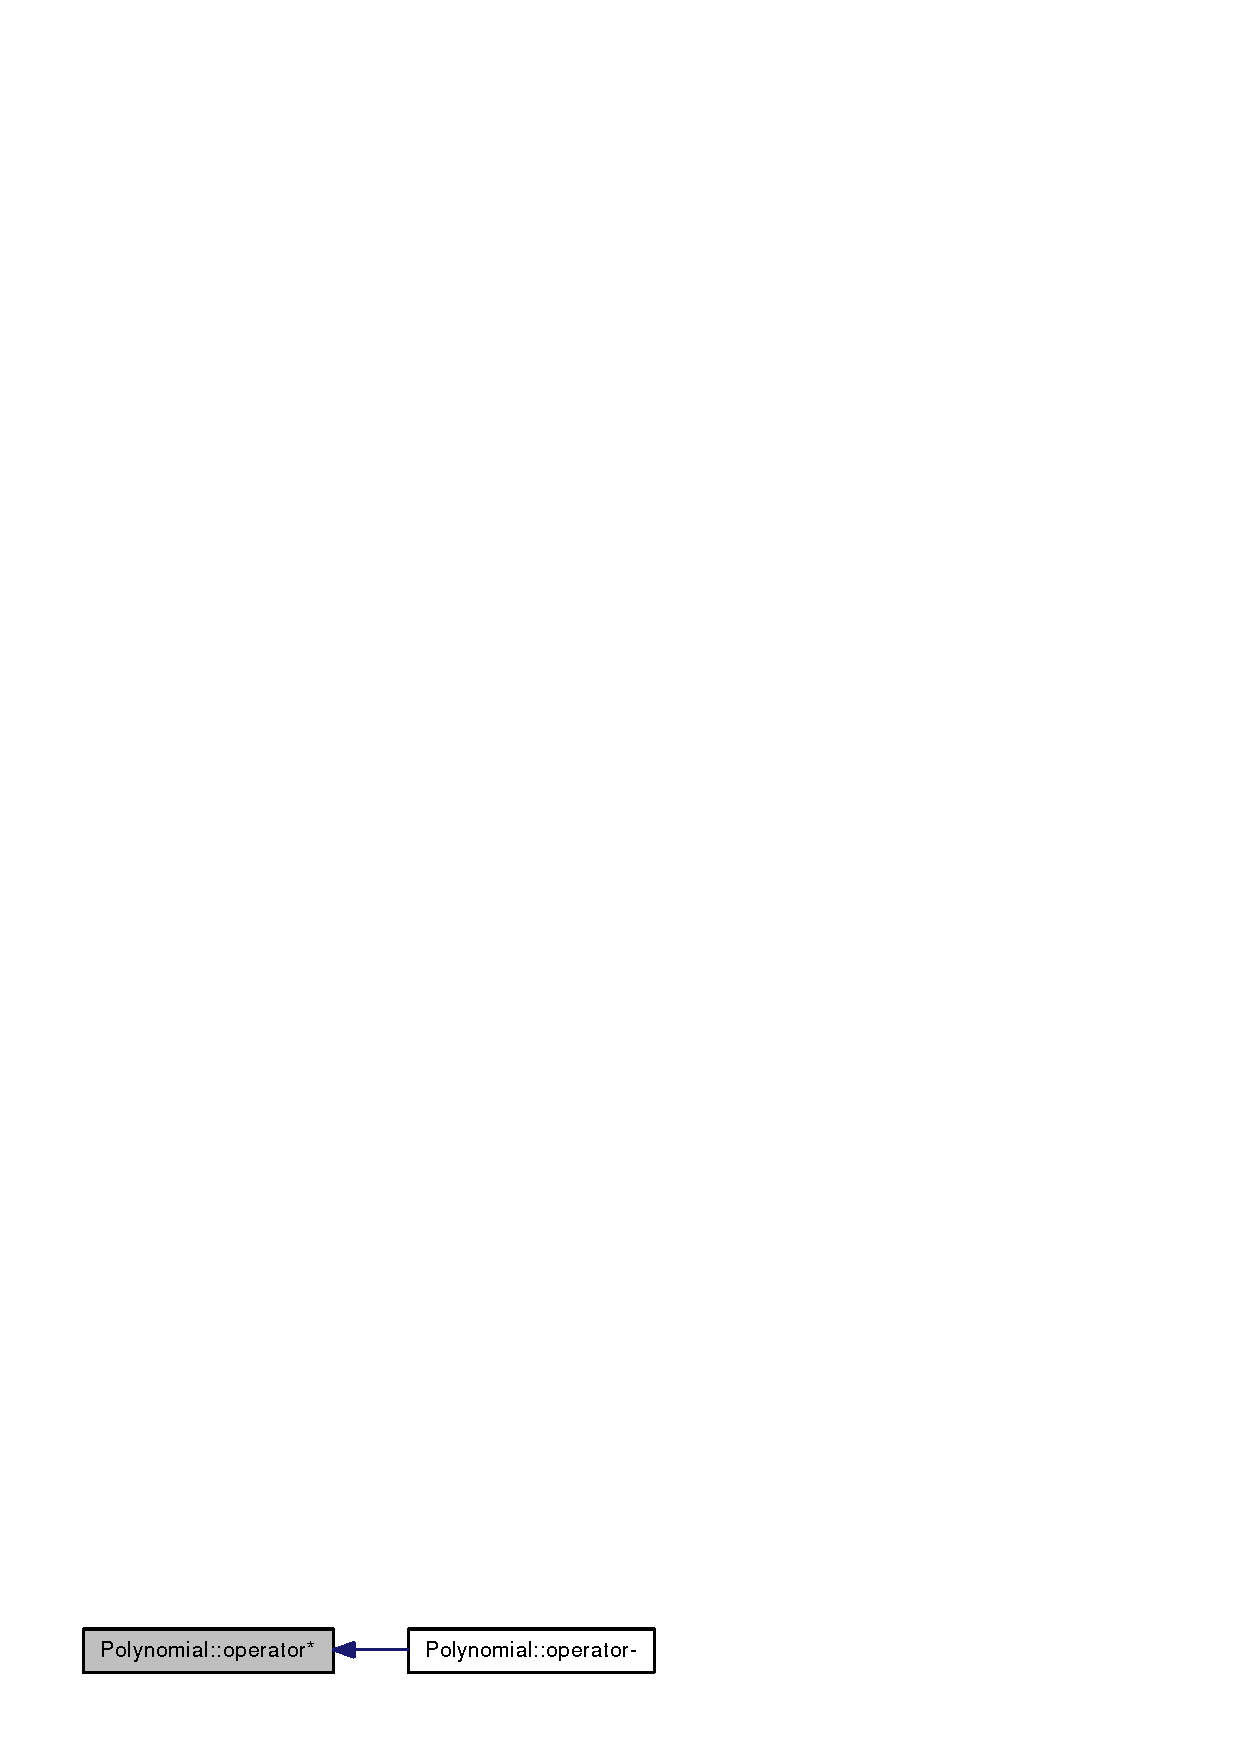
\includegraphics[width=159pt]{classPolynomial_1e00f25b4de1d335f437749c7bd93ac9_icgraph}
\end{center}
\end{figure}
\hypertarget{classPolynomial_cd98d02bf606b1f1cd7503d7e3b295a6}{
\index{Polynomial@{Polynomial}!operator$\ast$=@{operator$\ast$=}}
\index{operator$\ast$=@{operator$\ast$=}!Polynomial@{Polynomial}}
\subsubsection[operator$\ast$=]{\setlength{\rightskip}{0pt plus 5cm}{\bf Polynomial} \& Polynomial::operator$\ast$= (const {\bf Polynomial} \& {\em rhs})}}
\label{classPolynomial_cd98d02bf606b1f1cd7503d7e3b295a6}


multiplication/assignment operator 

Definition at line 171 of file poly.cc.

\begin{Code}\begin{verbatim}171                                                         {
172   *this = *this * rhs;
173   return *this;
174 }
\end{verbatim}
\end{Code}


\hypertarget{classPolynomial_d052b311f23798bf5136bd7444fd91d2}{
\index{Polynomial@{Polynomial}!operator-@{operator-}}
\index{operator-@{operator-}!Polynomial@{Polynomial}}
\subsubsection[operator-]{\setlength{\rightskip}{0pt plus 5cm}{\bf Polynomial} Polynomial::operator- () const}}
\label{classPolynomial_d052b311f23798bf5136bd7444fd91d2}


unary negation

unary negation operator just multiply by a scalar -1 

Definition at line 179 of file poly.cc.

References operator$\ast$().

\begin{Code}\begin{verbatim}180 {
181   return this->operator*(-1.0);
182 }
\end{verbatim}
\end{Code}




Here is the call graph for this function:\nopagebreak
\begin{figure}[H]
\begin{center}
\leavevmode
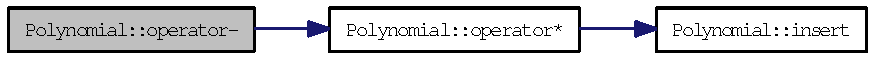
\includegraphics[width=228pt]{classPolynomial_d052b311f23798bf5136bd7444fd91d2_cgraph}
\end{center}
\end{figure}
\hypertarget{classPolynomial_c6eae37f11f87b541fa430de3643a31a}{
\index{Polynomial@{Polynomial}!operator()@{operator()}}
\index{operator()@{operator()}!Polynomial@{Polynomial}}
\subsubsection[operator()]{\setlength{\rightskip}{0pt plus 5cm}double Polynomial::operator() (double {\em a}) const}}
\label{classPolynomial_c6eae37f11f87b541fa430de3643a31a}


polynomial evaluation at a point a

evaluate at point a 

Definition at line 117 of file poly.cc.

References polynomial.

\begin{Code}\begin{verbatim}118 {
119   Polynomial p;
120   term *t, *u;
121   unsigned degree;
122   double result = 0;
123   // first reverse order the list
124   // since the polynomial is sorted,
125   // just peel off to the front each time.
126   t = polynomial;
127   while (t){
128     u =  p.polynomial;
129     p.polynomial = new term(*t);
130     t = t->next;
131     p.polynomial->next = u;
132   }
133   // seed with the highest order term
134   t = p.polynomial;
135   degree = t->deg;
136   // now evaluate the polynomial at a
137   while(t){
138     // multiply result by a
139     while(degree > t->deg){
140       result *= a;
141       degree--;
142     }
143     // add next coefficient
144     result += t->coef;
145     //remember depth (there might be gaps)
146     degree = t->deg;
147     // advance
148     t = t->next;
149   }
150   return result;
151 }
\end{verbatim}
\end{Code}


\hypertarget{classPolynomial_2ceb25a673d4c03b346595639ade0981}{
\index{Polynomial@{Polynomial}!operator+=@{operator+=}}
\index{operator+=@{operator+=}!Polynomial@{Polynomial}}
\subsubsection[operator+=]{\setlength{\rightskip}{0pt plus 5cm}{\bf Polynomial} \& Polynomial::operator+= (const {\bf Polynomial} \& {\em rhs})}}
\label{classPolynomial_2ceb25a673d4c03b346595639ade0981}


addition/assignment 

Definition at line 94 of file poly.cc.

References insert(), and polynomial.

\begin{Code}\begin{verbatim}95 {
96   Polynomial tmp(*this);
97   term * t = other.polynomial;
98   while(t){
99     tmp.insert(t->coef,t->deg);
100     t=t->next;
101   }
102   swap(tmp);
103   return *this;
104 }
\end{verbatim}
\end{Code}




Here is the call graph for this function:\nopagebreak
\begin{figure}[H]
\begin{center}
\leavevmode
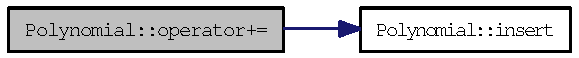
\includegraphics[width=157pt]{classPolynomial_2ceb25a673d4c03b346595639ade0981_cgraph}
\end{center}
\end{figure}
\hypertarget{classPolynomial_1e8588431fc5799e62bba71368a7234d}{
\index{Polynomial@{Polynomial}!abs@{abs}}
\index{abs@{abs}!Polynomial@{Polynomial}}
\subsubsection[abs]{\setlength{\rightskip}{0pt plus 5cm}{\bf Polynomial} Polynomial::abs () const}}
\label{classPolynomial_1e8588431fc5799e62bba71368a7234d}


make all coefficients positive 

Definition at line 213 of file poly.cc.

References polynomial.

\begin{Code}\begin{verbatim}213                                 {
214   Polynomial tmp(*this);
215   term *t = tmp.polynomial;
216   while(t){
217     if (t->coef <  0)
218       t->coef *= -1;
219     t = t->next;
220   }
221   return tmp;
222 }
\end{verbatim}
\end{Code}




Here is the caller graph for this function:\nopagebreak
\begin{figure}[H]
\begin{center}
\leavevmode
\includegraphics[width=103pt]{classPolynomial_1e8588431fc5799e62bba71368a7234d_icgraph}
\end{center}
\end{figure}
\hypertarget{classPolynomial_4db9e4f680c52fb8af45f3ae985a4055}{
\index{Polynomial@{Polynomial}!antiderivative@{antiderivative}}
\index{antiderivative@{antiderivative}!Polynomial@{Polynomial}}
\subsubsection[antiderivative]{\setlength{\rightskip}{0pt plus 5cm}{\bf Polynomial} Polynomial::antiderivative () const}}
\label{classPolynomial_4db9e4f680c52fb8af45f3ae985a4055}


general antiderivative with no arbitrary constant. Really, the arbitrary constant is zero here. by ignoring the constant we lose any meaningful result from antiderivative(0) which would have been a constant, but chooses 0 hence applying twice to 0, which would have been an arbitrary constant times x + another arbitrary constant, gives 0 for both constants, and looks like 0 again 

Definition at line 230 of file poly.cc.

References insert().

\begin{Code}\begin{verbatim}230                                             {
231   Polynomial p;
232   term *t = polynomial;
233   while(t){
234     if(t->deg == 0)
235       p.insert(t->coef, 1);
236     else
237       p.insert( t->coef /(1.0+ t->deg), t->deg+1);
238     t=t->next;
239   }
240   return p;
241 }
\end{verbatim}
\end{Code}




Here is the call graph for this function:\nopagebreak
\begin{figure}[H]
\begin{center}
\leavevmode
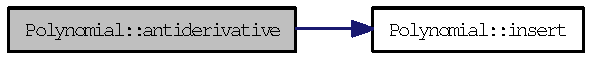
\includegraphics[width=160pt]{classPolynomial_4db9e4f680c52fb8af45f3ae985a4055_cgraph}
\end{center}
\end{figure}


Here is the caller graph for this function:\nopagebreak
\begin{figure}[H]
\begin{center}
\leavevmode
\includegraphics[width=150pt]{classPolynomial_4db9e4f680c52fb8af45f3ae985a4055_icgraph}
\end{center}
\end{figure}
\hypertarget{classPolynomial_aef1ed2dbc29d419c58c6d61b35853c3}{
\index{Polynomial@{Polynomial}!derivative@{derivative}}
\index{derivative@{derivative}!Polynomial@{Polynomial}}
\subsubsection[derivative]{\setlength{\rightskip}{0pt plus 5cm}{\bf Polynomial} Polynomial::derivative () const}}
\label{classPolynomial_aef1ed2dbc29d419c58c6d61b35853c3}


derivative as a polynomial 

Definition at line 196 of file poly.cc.

References insert().

\begin{Code}\begin{verbatim}196                                         {
197   Polynomial p;
198   term *t = polynomial;
199   while(t){
200     if(t->deg)
201       p.insert((t->coef * t->deg), t->deg - 1);
202     t = t->next;
203   }
204   return p;
205 }
\end{verbatim}
\end{Code}




Here is the call graph for this function:\nopagebreak
\begin{figure}[H]
\begin{center}
\leavevmode
\includegraphics[width=151pt]{classPolynomial_aef1ed2dbc29d419c58c6d61b35853c3_cgraph}
\end{center}
\end{figure}


Here is the caller graph for this function:\nopagebreak
\begin{figure}[H]
\begin{center}
\leavevmode
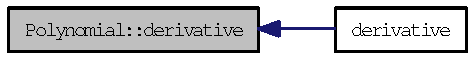
\includegraphics[width=132pt]{classPolynomial_aef1ed2dbc29d419c58c6d61b35853c3_icgraph}
\end{center}
\end{figure}


\subsection{Friends And Related Function Documentation}
\hypertarget{classPolynomial_1446b464245742ccedeacb27fd794bab}{
\index{Polynomial@{Polynomial}!operator$>$$>$@{operator$>$$>$}}
\index{operator$>$$>$@{operator$>$$>$}!Polynomial@{Polynomial}}
\subsubsection[operator$>$$>$]{\setlength{\rightskip}{0pt plus 5cm}std::istream\& operator$>$$>$ (std::istream \& {\em is}, \/  {\bf Polynomial} \& {\em p})\hspace{0.3cm}{\tt  \mbox{[}friend\mbox{]}}}}
\label{classPolynomial_1446b464245742ccedeacb27fd794bab}


extraction operator to read polynomials

extraction operator get a pair of numbers double, unsigned from an istream This might not be the best way to do this, and is nowhere used. 

Definition at line 340 of file poly.cc.

\begin{Code}\begin{verbatim}340                                                      {
341   double coef;
342   unsigned int  degree;
343   Polynomial::term *t;
344   coef = 0.0;
345   while (coef == 0.0){
346     is>>coef;
347     is>>degree;
348     if(!is.fail()){
349       t = new Polynomial::term(coef, degree);
350       p.insert(t);
351     }
352   }
353   return is;
354 }
\end{verbatim}
\end{Code}


\hypertarget{classPolynomial_f1fdf53b29100b084772816cb9ecc8ac}{
\index{Polynomial@{Polynomial}!operator$<$$<$@{operator$<$$<$}}
\index{operator$<$$<$@{operator$<$$<$}!Polynomial@{Polynomial}}
\subsubsection[operator$<$$<$]{\setlength{\rightskip}{0pt plus 5cm}std::ostream\& operator$<$$<$ (std::ostream \& {\em os}, \/  const {\bf Polynomial} \& {\em p})\hspace{0.3cm}{\tt  \mbox{[}friend\mbox{]}}}}
\label{classPolynomial_f1fdf53b29100b084772816cb9ecc8ac}


insertion operator to print polynomials

operator$<$$<$ insert polynomial into an output stream terms will be printed in order of increasing degree 

Definition at line 309 of file poly.cc.

\begin{Code}\begin{verbatim}309                                                            {
310   Polynomial::term * t;
311   t = p.polynomial;
312   bool first = true;
313   while(t){
314     if(t->coef != 0.0){
315       if(!first)
316     os<<" + ";
317 
318       os<< t->coef;
319       if(t->deg){
320     os<<"*x";
321     if(t->deg > 1)
322       os<<"^"<<t->deg;
323       }
324       //    os<<" ";
325     first = false;
326    }
327     t = t->next;
328 
329   }
330   if (first)
331     os<<"0";
332   return os;
333 }
\end{verbatim}
\end{Code}




The documentation for this class was generated from the following files:\begin{CompactItemize}
\item 
\hyperlink{poly_8h}{poly.h}\item 
\hyperlink{poly_8cc}{poly.cc}\end{CompactItemize}

\hypertarget{classPolynomialMenu}{
\section{PolynomialMenu Class Reference}
\label{classPolynomialMenu}\index{PolynomialMenu@{PolynomialMenu}}
}
The main program logic, contains a vector of Polynomials, means to generate them, means to add and multiply existing polynomials, handles user input/output, and displays the menu and the polynomials in the vector.  


{\tt \#include $<$menu.h$>$}

Collaboration diagram for PolynomialMenu:\nopagebreak
\begin{figure}[H]
\begin{center}
\leavevmode
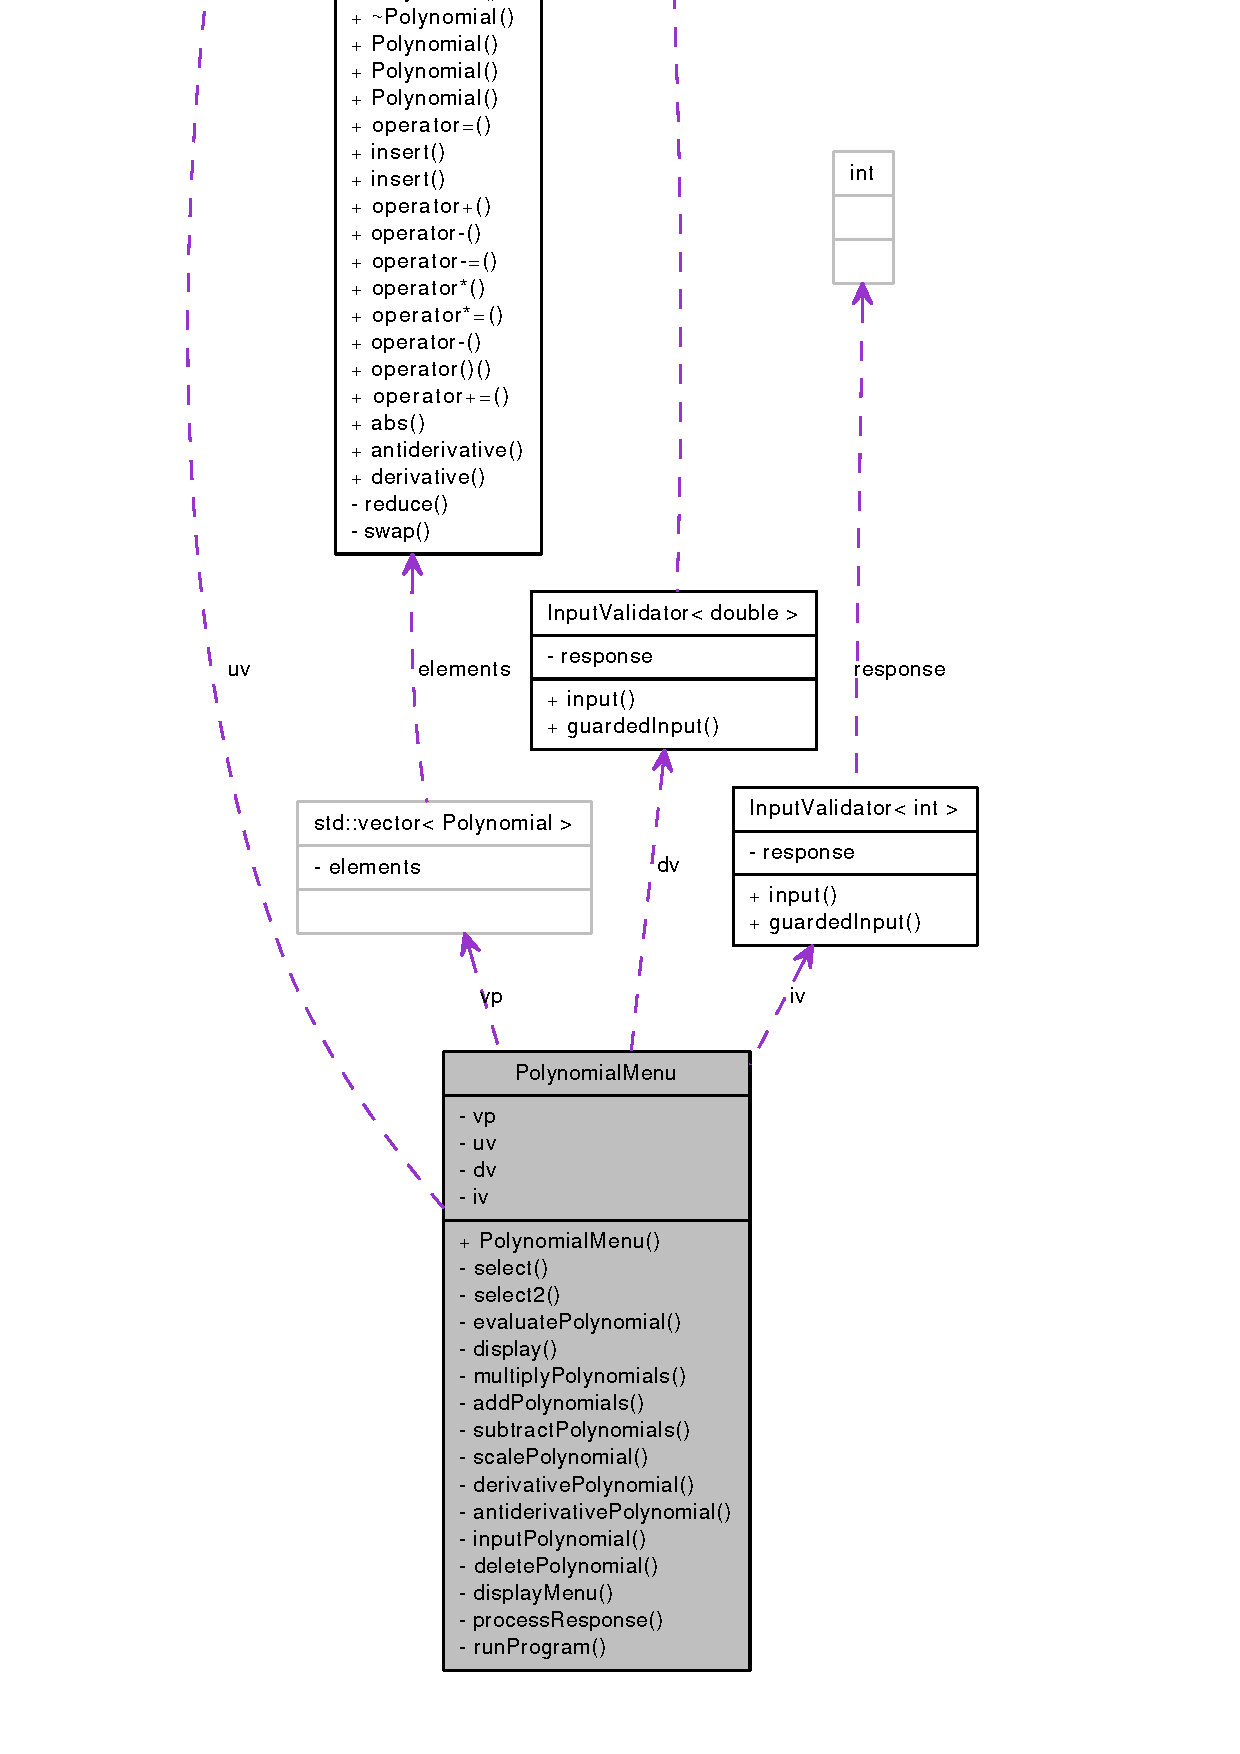
\includegraphics[width=400pt]{classPolynomialMenu__coll__graph}
\end{center}
\end{figure}
\subsection*{Public Member Functions}
\begin{CompactItemize}
\item 
\hyperlink{classPolynomialMenu_bcc711635d8721ea6803a73a706ff47e}{PolynomialMenu} ()
\end{CompactItemize}


\subsection{Detailed Description}
The main program logic, contains a vector of Polynomials, means to generate them, means to add and multiply existing polynomials, handles user input/output, and displays the menu and the polynomials in the vector. 

This is less a proper object than a grouping of related functions, the class mechanism was used to share what otherwise would have been global variables (vector of polynomials), or commonly reused items in many functions (input validator objects). 

Definition at line 28 of file menu.h.

\subsection{Constructor \& Destructor Documentation}
\hypertarget{classPolynomialMenu_bcc711635d8721ea6803a73a706ff47e}{
\index{PolynomialMenu@{PolynomialMenu}!PolynomialMenu@{PolynomialMenu}}
\index{PolynomialMenu@{PolynomialMenu}!PolynomialMenu@{PolynomialMenu}}
\subsubsection[PolynomialMenu]{\setlength{\rightskip}{0pt plus 5cm}PolynomialMenu::PolynomialMenu ()}}
\label{classPolynomialMenu_bcc711635d8721ea6803a73a706ff47e}


Constructor calls runProgram 

Definition at line 192 of file menu.cc.

\begin{Code}\begin{verbatim}192                               {
193   runProgram();
194 }
\end{verbatim}
\end{Code}




The documentation for this class was generated from the following files:\begin{CompactItemize}
\item 
\hyperlink{menu_8h}{menu.h}\item 
\hyperlink{menu_8cc}{menu.cc}\end{CompactItemize}

\chapter{File Documentation}
\hypertarget{InputValidator_8h}{
\section{InputValidator.h File Reference}
\label{InputValidator_8h}\index{InputValidator.h@{InputValidator.h}}
}
A templated type validator from cin/cout. 

{\tt \#include $<$iostream$>$}\par
{\tt \#include $<$string$>$}\par


Include dependency graph for InputValidator.h:\nopagebreak
\begin{figure}[H]
\begin{center}
\leavevmode
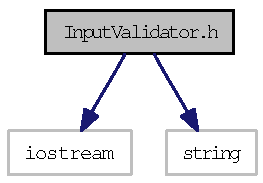
\includegraphics[width=81pt]{InputValidator_8h__incl}
\end{center}
\end{figure}


This graph shows which files directly or indirectly include this file:\nopagebreak
\begin{figure}[H]
\begin{center}
\leavevmode
\includegraphics[width=86pt]{InputValidator_8h__dep__incl}
\end{center}
\end{figure}
\subsection*{Classes}
\begin{CompactItemize}
\item 
class \hyperlink{classInputValidator}{InputValidator$<$ T $>$}
\end{CompactItemize}


\subsection{Detailed Description}
A templated type validator from cin/cout. 

\begin{Desc}
\item[Author:]Daniel Uber \end{Desc}


Definition in file \hyperlink{InputValidator_8h-source}{InputValidator.h}.
\hypertarget{main_8cc}{
\section{main.cc File Reference}
\label{main_8cc}\index{main.cc@{main.cc}}
}
Start menu system. 

{\tt \#include \char`\"{}menu.h\char`\"{}}\par


Include dependency graph for main.cc:\nopagebreak
\begin{figure}[H]
\begin{center}
\leavevmode
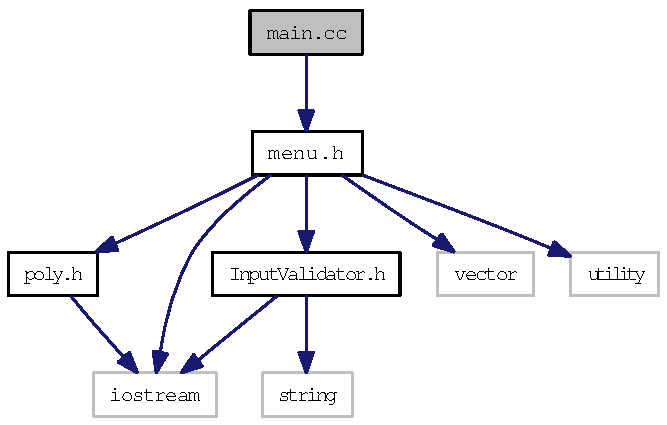
\includegraphics[width=178pt]{main_8cc__incl}
\end{center}
\end{figure}
\subsection*{Functions}
\begin{CompactItemize}
\item 
int \hyperlink{main_8cc_51af30a60f9f02777c6396b8247e356f}{main} ()
\end{CompactItemize}


\subsection{Detailed Description}
Start menu system. 

\begin{Desc}
\item[Author:]Daniel Uber \end{Desc}


Definition in file \hyperlink{main_8cc-source}{main.cc}.

\subsection{Function Documentation}
\hypertarget{main_8cc_51af30a60f9f02777c6396b8247e356f}{
\index{main.cc@{main.cc}!main@{main}}
\index{main@{main}!main.cc@{main.cc}}
\subsubsection[main]{\setlength{\rightskip}{0pt plus 5cm}main ()}}
\label{main_8cc_51af30a60f9f02777c6396b8247e356f}


simple program logic, creates a self starting menu object 

Definition at line 12 of file main.cc.

\begin{Code}\begin{verbatim}12           {
13   PolynomialMenu m;
14   return 0;
15  }
\end{verbatim}
\end{Code}



\hypertarget{menu_8cc}{
\section{menu.cc File Reference}
\label{menu_8cc}\index{menu.cc@{menu.cc}}
}
implement the menu logic 

{\tt \#include \char`\"{}menu.h\char`\"{}}\par


Include dependency graph for menu.cc:\nopagebreak
\begin{figure}[H]
\begin{center}
\leavevmode
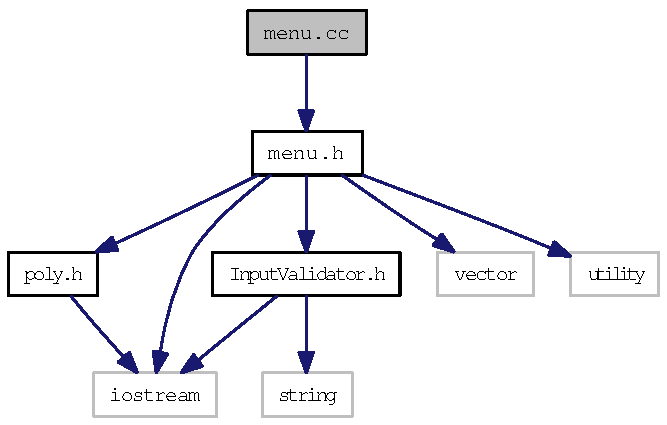
\includegraphics[width=178pt]{menu_8cc__incl}
\end{center}
\end{figure}


\subsection{Detailed Description}
implement the menu logic 

\begin{Desc}
\item[Author:]Daniel Uber \end{Desc}


Definition in file \hyperlink{menu_8cc-source}{menu.cc}.
\hypertarget{menu_8h}{
\section{menu.h File Reference}
\label{menu_8h}\index{menu.h@{menu.h}}
}
definition of the polynomial menu system 

{\tt \#include \char`\"{}poly.h\char`\"{}}\par
{\tt \#include \char`\"{}InputValidator.h\char`\"{}}\par
{\tt \#include $<$iostream$>$}\par
{\tt \#include $<$vector$>$}\par
{\tt \#include $<$utility$>$}\par


Include dependency graph for menu.h:\nopagebreak
\begin{figure}[H]
\begin{center}
\leavevmode
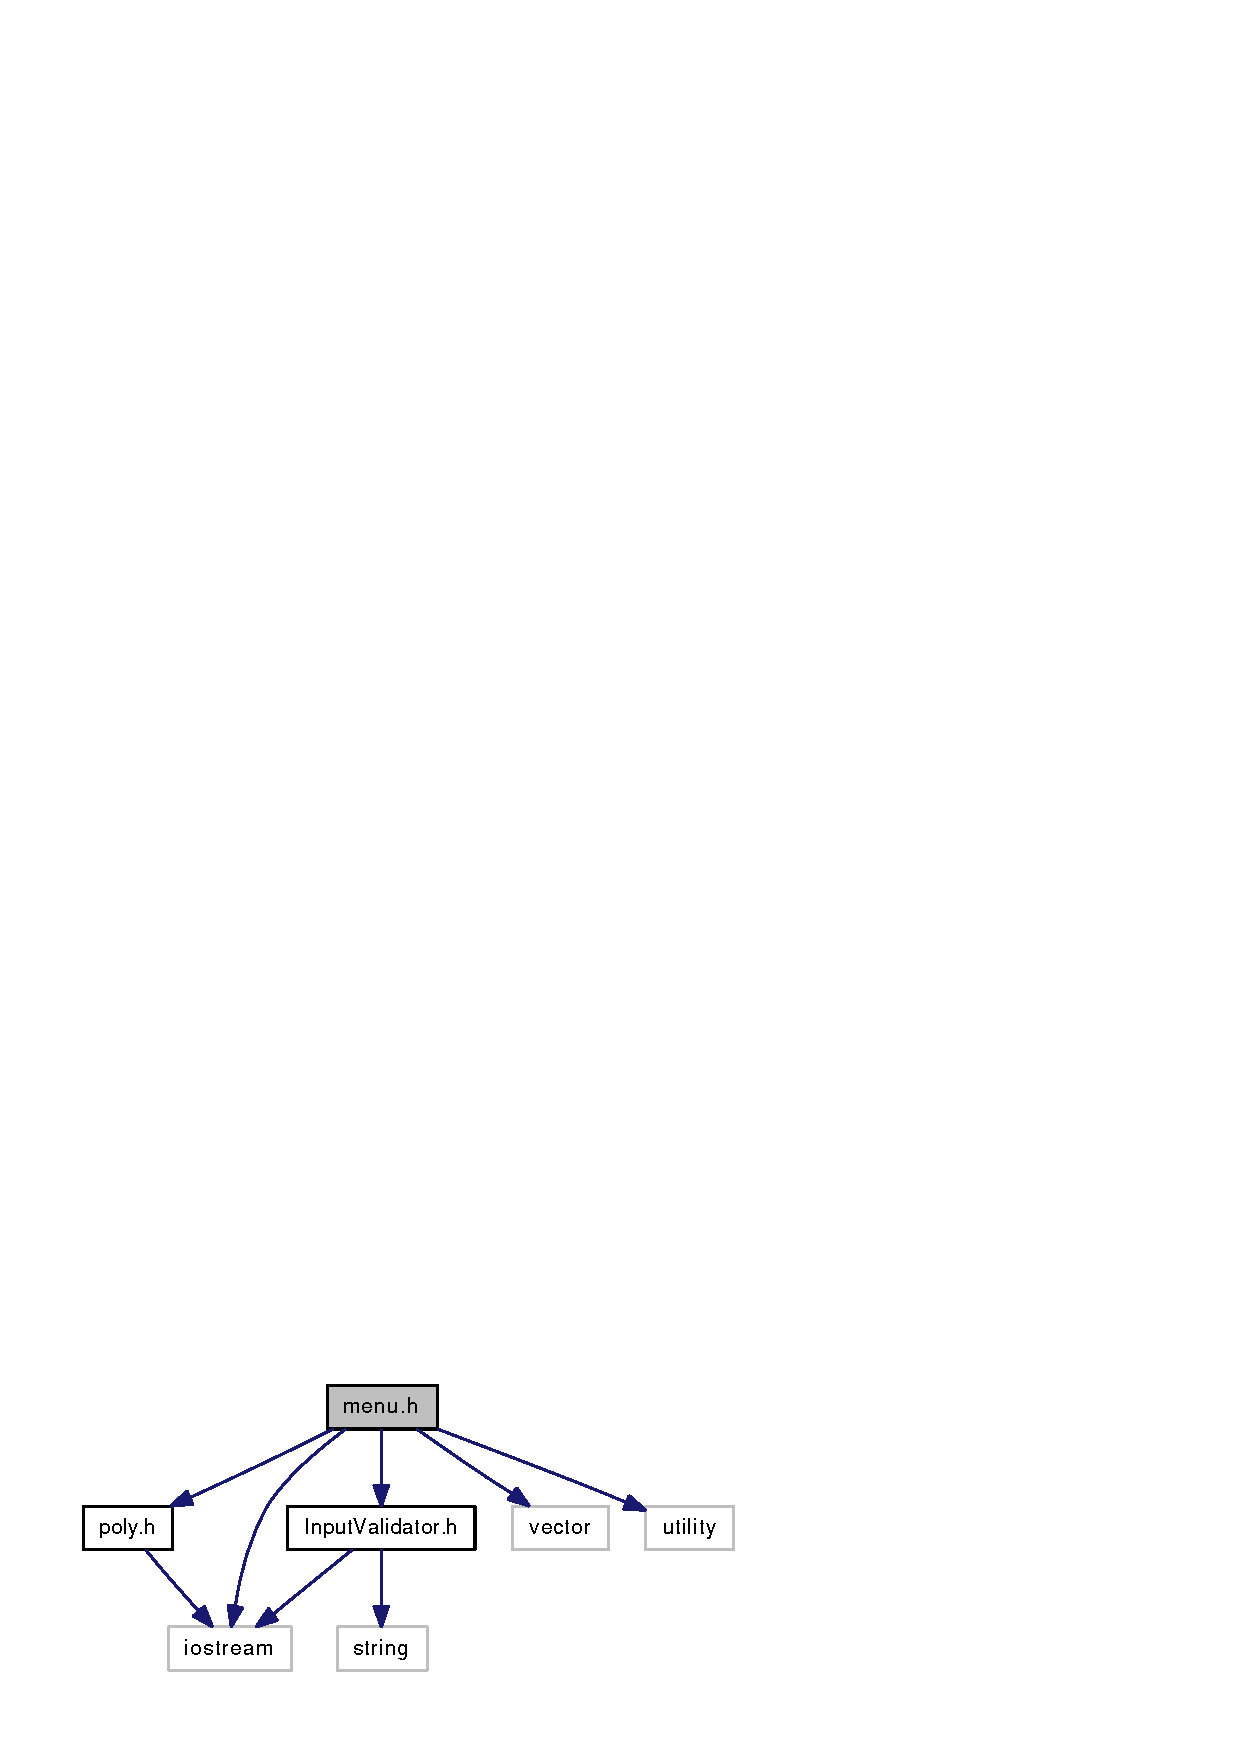
\includegraphics[width=178pt]{menu_8h__incl}
\end{center}
\end{figure}


This graph shows which files directly or indirectly include this file:\nopagebreak
\begin{figure}[H]
\begin{center}
\leavevmode
\includegraphics[width=86pt]{menu_8h__dep__incl}
\end{center}
\end{figure}
\subsection*{Classes}
\begin{CompactItemize}
\item 
class \hyperlink{classPolynomialMenu}{PolynomialMenu}
\begin{CompactList}\small\item\em The main program logic, contains a vector of Polynomials, means to generate them, means to add and multiply existing polynomials, handles user input/output, and displays the menu and the polynomials in the vector. \item\end{CompactList}\end{CompactItemize}


\subsection{Detailed Description}
definition of the polynomial menu system 

\begin{Desc}
\item[Author:]Daniel Uber \end{Desc}


Definition in file \hyperlink{menu_8h-source}{menu.h}.
\hypertarget{poly_8cc}{
\section{poly.cc File Reference}
\label{poly_8cc}\index{poly.cc@{poly.cc}}
}
Implementation for the polynomial class. 

{\tt \#include \char`\"{}poly.h\char`\"{}}\par
{\tt \#include $<$cstring$>$}\par


Include dependency graph for poly.cc:\nopagebreak
\begin{figure}[H]
\begin{center}
\leavevmode
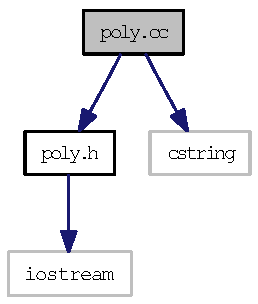
\includegraphics[width=80pt]{poly_8cc__incl}
\end{center}
\end{figure}
\subsection*{Functions}
\begin{CompactItemize}
\item 
\hyperlink{classPolynomial}{Polynomial} \hyperlink{poly_8cc_45b456660c9d558815a111d3d7c5a807}{derivative} (const \hyperlink{classPolynomial}{Polynomial} \&p)
\item 
\hyperlink{classPolynomial}{Polynomial} \hyperlink{poly_8cc_55bc2f7d47ec37dcd68435f19fa083cc}{abs} (const \hyperlink{classPolynomial}{Polynomial} \&p)
\item 
\hyperlink{classPolynomial}{Polynomial} \hyperlink{poly_8cc_aeb620028554ea52c7716904a27a7cd6}{antiderivative} (const \hyperlink{classPolynomial}{Polynomial} \&p)
\item 
std::ostream \& \hyperlink{poly_8cc_f1fdf53b29100b084772816cb9ecc8ac}{operator$<$$<$} (std::ostream \&os, const \hyperlink{classPolynomial}{Polynomial} \&p)
\item 
std::istream \& \hyperlink{poly_8cc_1446b464245742ccedeacb27fd794bab}{operator$>$$>$} (std::istream \&is, \hyperlink{classPolynomial}{Polynomial} \&p)
\end{CompactItemize}


\subsection{Detailed Description}
Implementation for the polynomial class. 

\begin{Desc}
\item[Author:]Daniel Uber \end{Desc}


Definition in file \hyperlink{poly_8cc-source}{poly.cc}.

\subsection{Function Documentation}
\hypertarget{poly_8cc_55bc2f7d47ec37dcd68435f19fa083cc}{
\index{poly.cc@{poly.cc}!abs@{abs}}
\index{abs@{abs}!poly.cc@{poly.cc}}
\subsubsection[abs]{\setlength{\rightskip}{0pt plus 5cm}abs (const {\bf Polynomial} \& {\em p})}}
\label{poly_8cc_55bc2f7d47ec37dcd68435f19fa083cc}


\begin{Desc}
\item[Returns:]absolute value of polynomial \end{Desc}


Definition at line 226 of file poly.cc.

References Polynomial::abs().

\begin{Code}\begin{verbatim}226                                    {
227   return p.abs();
228 }
\end{verbatim}
\end{Code}




Here is the call graph for this function:\nopagebreak
\begin{figure}[H]
\begin{center}
\leavevmode
\includegraphics[width=103pt]{poly_8cc_55bc2f7d47ec37dcd68435f19fa083cc_cgraph}
\end{center}
\end{figure}
\hypertarget{poly_8cc_aeb620028554ea52c7716904a27a7cd6}{
\index{poly.cc@{poly.cc}!antiderivative@{antiderivative}}
\index{antiderivative@{antiderivative}!poly.cc@{poly.cc}}
\subsubsection[antiderivative]{\setlength{\rightskip}{0pt plus 5cm}antiderivative (const {\bf Polynomial} \& {\em p})}}
\label{poly_8cc_aeb620028554ea52c7716904a27a7cd6}


\begin{Desc}
\item[Returns:]indefinite integral of p with constant 0 \end{Desc}


Definition at line 245 of file poly.cc.

References Polynomial::antiderivative().

\begin{Code}\begin{verbatim}245                                                 {
246   return p.antiderivative();
247 }
\end{verbatim}
\end{Code}




Here is the call graph for this function:\nopagebreak
\begin{figure}[H]
\begin{center}
\leavevmode
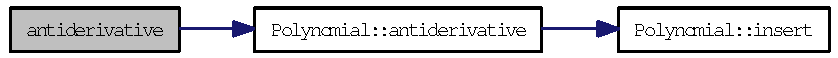
\includegraphics[width=219pt]{poly_8cc_aeb620028554ea52c7716904a27a7cd6_cgraph}
\end{center}
\end{figure}
\hypertarget{poly_8cc_45b456660c9d558815a111d3d7c5a807}{
\index{poly.cc@{poly.cc}!derivative@{derivative}}
\index{derivative@{derivative}!poly.cc@{poly.cc}}
\subsubsection[derivative]{\setlength{\rightskip}{0pt plus 5cm}derivative (const {\bf Polynomial} \& {\em p})}}
\label{poly_8cc_45b456660c9d558815a111d3d7c5a807}


return polynomial derivative 

Definition at line 209 of file poly.cc.

References Polynomial::derivative().

\begin{Code}\begin{verbatim}209                                            {
210   return p.derivative();
211 }
\end{verbatim}
\end{Code}




Here is the call graph for this function:\nopagebreak
\begin{figure}[H]
\begin{center}
\leavevmode
\includegraphics[width=201pt]{poly_8cc_45b456660c9d558815a111d3d7c5a807_cgraph}
\end{center}
\end{figure}
\hypertarget{poly_8cc_f1fdf53b29100b084772816cb9ecc8ac}{
\index{poly.cc@{poly.cc}!operator$<$$<$@{operator$<$$<$}}
\index{operator$<$$<$@{operator$<$$<$}!poly.cc@{poly.cc}}
\subsubsection[operator$<$$<$]{\setlength{\rightskip}{0pt plus 5cm}std::ostream\& operator$<$$<$ (std::ostream \& {\em os}, \/  const {\bf Polynomial} \& {\em p})}}
\label{poly_8cc_f1fdf53b29100b084772816cb9ecc8ac}


operator$<$$<$ insert polynomial into an output stream terms will be printed in order of increasing degree 

Definition at line 309 of file poly.cc.

References Polynomial::polynomial.

\begin{Code}\begin{verbatim}309                                                            {
310   Polynomial::term * t;
311   t = p.polynomial;
312   bool first = true;
313   while(t){
314     if(t->coef != 0.0){
315       if(!first)
316     os<<" + ";
317 
318       os<< t->coef;
319       if(t->deg){
320     os<<"*x";
321     if(t->deg > 1)
322       os<<"^"<<t->deg;
323       }
324       //    os<<" ";
325     first = false;
326    }
327     t = t->next;
328 
329   }
330   if (first)
331     os<<"0";
332   return os;
333 }
\end{verbatim}
\end{Code}


\hypertarget{poly_8cc_1446b464245742ccedeacb27fd794bab}{
\index{poly.cc@{poly.cc}!operator$>$$>$@{operator$>$$>$}}
\index{operator$>$$>$@{operator$>$$>$}!poly.cc@{poly.cc}}
\subsubsection[operator$>$$>$]{\setlength{\rightskip}{0pt plus 5cm}std::istream\& operator$>$$>$ (std::istream \& {\em is}, \/  {\bf Polynomial} \& {\em p})}}
\label{poly_8cc_1446b464245742ccedeacb27fd794bab}


extraction operator get a pair of numbers double, unsigned from an istream This might not be the best way to do this, and is nowhere used. 

Definition at line 340 of file poly.cc.

References Polynomial::insert().

\begin{Code}\begin{verbatim}340                                                      {
341   double coef;
342   unsigned int  degree;
343   Polynomial::term *t;
344   coef = 0.0;
345   while (coef == 0.0){
346     is>>coef;
347     is>>degree;
348     if(!is.fail()){
349       t = new Polynomial::term(coef, degree);
350       p.insert(t);
351     }
352   }
353   return is;
354 }
\end{verbatim}
\end{Code}




Here is the call graph for this function:\nopagebreak
\begin{figure}[H]
\begin{center}
\leavevmode
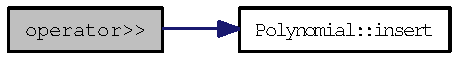
\includegraphics[width=128pt]{poly_8cc_1446b464245742ccedeacb27fd794bab_cgraph}
\end{center}
\end{figure}

\hypertarget{poly_8h}{
\section{poly.h File Reference}
\label{poly_8h}\index{poly.h@{poly.h}}
}
Declaration of the polynomial class. 

{\tt \#include $<$iostream$>$}\par


Include dependency graph for poly.h:\nopagebreak
\begin{figure}[H]
\begin{center}
\leavevmode
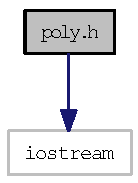
\includegraphics[width=51pt]{poly_8h__incl}
\end{center}
\end{figure}


This graph shows which files directly or indirectly include this file:\nopagebreak
\begin{figure}[H]
\begin{center}
\leavevmode
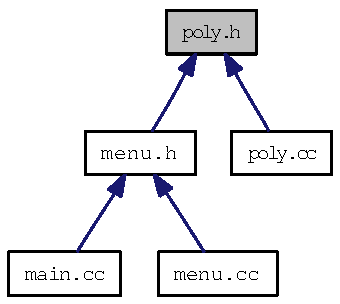
\includegraphics[width=99pt]{poly_8h__dep__incl}
\end{center}
\end{figure}
\subsection*{Classes}
\begin{CompactItemize}
\item 
class \hyperlink{classPolynomial}{Polynomial}
\begin{CompactList}\small\item\em represents the polynomial as a linked list of terms \item\end{CompactList}\item 
class \textbf{Polynomial::term}
\end{CompactItemize}
\subsection*{Functions}
\begin{CompactItemize}
\item 
\hyperlink{classPolynomial}{Polynomial} \hyperlink{poly_8h_a5dcabab23da371f543b0daccb699b9d}{abs} (const \hyperlink{classPolynomial}{Polynomial} \&p)
\item 
\hyperlink{classPolynomial}{Polynomial} \hyperlink{poly_8h_b201f37e58ec35c0d6fc0029ea309a92}{derivative} (const \hyperlink{classPolynomial}{Polynomial} \&p)
\item 
\hyperlink{classPolynomial}{Polynomial} \hyperlink{poly_8h_a512be609af2a7ca60e6ae4fbca63421}{antiderivative} (const \hyperlink{classPolynomial}{Polynomial} \&p)
\end{CompactItemize}


\subsection{Detailed Description}
Declaration of the polynomial class. 

\begin{Desc}
\item[Author:]Daniel Uber \end{Desc}


Definition in file \hyperlink{poly_8h-source}{poly.h}.

\subsection{Function Documentation}
\hypertarget{poly_8h_a5dcabab23da371f543b0daccb699b9d}{
\index{poly.h@{poly.h}!abs@{abs}}
\index{abs@{abs}!poly.h@{poly.h}}
\subsubsection[abs]{\setlength{\rightskip}{0pt plus 5cm}{\bf Polynomial} abs (const {\bf Polynomial} \& {\em p})}}
\label{poly_8h_a5dcabab23da371f543b0daccb699b9d}


\begin{Desc}
\item[Returns:]absolute value of polynomial \end{Desc}


Definition at line 226 of file poly.cc.

References Polynomial::abs().

\begin{Code}\begin{verbatim}226                                    {
227   return p.abs();
228 }
\end{verbatim}
\end{Code}




Here is the call graph for this function:\nopagebreak
\begin{figure}[H]
\begin{center}
\leavevmode
\includegraphics[width=103pt]{poly_8h_a5dcabab23da371f543b0daccb699b9d_cgraph}
\end{center}
\end{figure}
\hypertarget{poly_8h_a512be609af2a7ca60e6ae4fbca63421}{
\index{poly.h@{poly.h}!antiderivative@{antiderivative}}
\index{antiderivative@{antiderivative}!poly.h@{poly.h}}
\subsubsection[antiderivative]{\setlength{\rightskip}{0pt plus 5cm}{\bf Polynomial} antiderivative (const {\bf Polynomial} \& {\em p})}}
\label{poly_8h_a512be609af2a7ca60e6ae4fbca63421}


\begin{Desc}
\item[Returns:]indefinite integral of p with constant 0 \end{Desc}


Definition at line 245 of file poly.cc.

References Polynomial::antiderivative().

\begin{Code}\begin{verbatim}245                                                 {
246   return p.antiderivative();
247 }
\end{verbatim}
\end{Code}




Here is the call graph for this function:\nopagebreak
\begin{figure}[H]
\begin{center}
\leavevmode
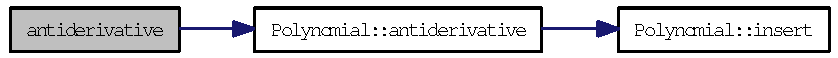
\includegraphics[width=219pt]{poly_8h_a512be609af2a7ca60e6ae4fbca63421_cgraph}
\end{center}
\end{figure}
\hypertarget{poly_8h_b201f37e58ec35c0d6fc0029ea309a92}{
\index{poly.h@{poly.h}!derivative@{derivative}}
\index{derivative@{derivative}!poly.h@{poly.h}}
\subsubsection[derivative]{\setlength{\rightskip}{0pt plus 5cm}{\bf Polynomial} derivative (const {\bf Polynomial} \& {\em p})}}
\label{poly_8h_b201f37e58ec35c0d6fc0029ea309a92}


return polynomial derivative 

Definition at line 209 of file poly.cc.

References Polynomial::derivative().

\begin{Code}\begin{verbatim}209                                            {
210   return p.derivative();
211 }
\end{verbatim}
\end{Code}




Here is the call graph for this function:\nopagebreak
\begin{figure}[H]
\begin{center}
\leavevmode
\includegraphics[width=201pt]{poly_8h_b201f37e58ec35c0d6fc0029ea309a92_cgraph}
\end{center}
\end{figure}

\printindex
\end{document}
